%% TITOLO
\section{Ecosistemi Udibili}
\label{sec:Ecosistemi Udibili}
%% TESTO
% - proseguire partendo dagli articoli di Agostino Di Scipio, da Polveri Sonore,
% dalle analisi musicali come quelle di Makis Solomos. Discutere gli elementi del
% sistema e il loro ruolo in Audible Ecosystemics 2 + Codici Faust degli agenti.
% In coda al capitolo rimandare al codice completo in Appendice A e plot
% grafici di Faust in Appendice B -

Uno degli esiti musicali più importanti che ha portato con sé 
il paradigma della complessità, riguarda essenzialmente l'aver smesso di 
scrivere musica per strumenti interattivi con cui farla e viceversa, 
ed esser passati invece al  comporre le interazioni tramite gli strumenti. \\
Le interazioni ho ritenuto importante affrontare sono di due tipi, 
di sistemi che interagiscono con l’ambiente circostante appartenente al mondo fisico, 
e sistemi che interagiscono con il proprio ambiente nel mondo digitale, 
ma prima di entrare nel merito è necessario spendere qualche parola sul cosa
si intenda qui per ambiente. \\
Nessun sistema è separabile e isolabile dall'ambiente circostante, 
a prescindere dal fatto che il suo spazio vitale, sia nel mondo fisico o digitale. 
Proprio come ha mostrato Heinz Von Foerster non si può parlare di auto-organizzazione
se non ci si riferisce essenzialmente a un ambiente che racchiude il sistema al suo interno. 
E in particolare, quello che si manifesta quando un sistema entra in interazione non distruttiva 
con l'ambiente circostante, che è sostanzialmente il suo spazio vitale, è un Ecosistema. \\
I lavori del ciclo Ecosistemico Udibile di Agostino di Scipio, in tal senso, 
trovano fondamento a partire da fenomeni e relazioni che possono esistere e manifestarsi solamente nell'ambiente circostante da cui prende vita il sistema, 
che in questo caso è proprio lo spazio acustico reale. 
Lavori come lo studio sul feedback, lo studio sul rumore di fondo, lo studio sulle risposte all'impulso, o
lo studio sul silenzio, sono nella loro essenza dei sistemi che hanno come seme 
della loro morfogenesi un determinato 
comportamento appartenente allo spazio acustico reale, delimitato in questi studi da una stanza
che ne racchiude al suo interno tutti gli agenti e le relazioni possibili,
per costruirne una storia di relazioni dove il sistema si osserva attraverso lo spazio fisico, 
(ambiente) e si manifesta e vive solo attraverso di esso.
In questo senso l’interprete, lo spazio, e gli ascoltatori, 
divengono essi stessi parte integrante del sistema, dove l’ascolto, diviene anche esso
parte dell’insieme delle cose e delle relazioni che lo costituisce. \\

\subsection{L'interazione Uomo-Macchina-Ambiente}
\label{sec:L'interazione Uomo-Macchina-Ambiente}

Qual'è dunque l'esigenza alla base del comporre le interazioni invece 
che limitarsi al comporre musica per strumenti interattivi? 
Superare la classica relazione uomo-macchina dominante nella tradizione musicale, 
iniziando a pensare invece allo sconfinato universo delle nuove possibilità della complessità.
Secondo Agostino Di Scipio, questo avviene in primo luogo grazie 
alla possibilità che la macchina possa rappresentarsi
senza mediazione umana, e attraverso l'ambiente circostante, \footcite{discipio_polverisonore_2016}
e dunque poi alla possibilità di stabilire un flusso di relazioni macchina-ambiente. 
Consentendo in secondo luogo al musicista e performer 
la possibilità di potersi aprire ad un flusso di relazioni 
complesso fra uomo-macchina-ambiente dove le tre sono fortamente connesse e interdipendenti 
l'una dall'altra.

\begin{center}
\vspace{0.5cm}
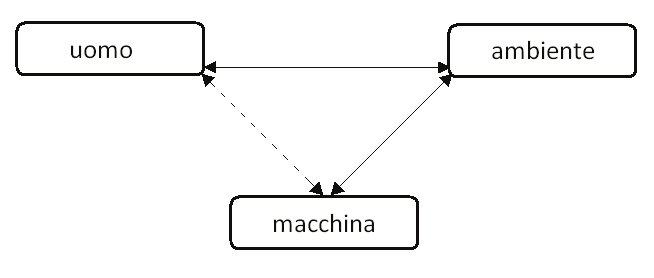
\includegraphics[width=8cm]{figures/uomo_macchina_ambiente.png} \\
{Interazione Uomo-Macchina-Ambiente} \\ 
\vspace{0.5cm}
\end{center}

\begin{center}
\vspace{0.5cm}
\textit{la mossa decisiva è: passare da un lavoro che mira a usare mezzi interattivi per creare forme sonore desiderate ad
un lavoro che mira a creare le interazioni desiderate e ad ascoltarne le tracce udibili. Nel secondo caso, si tratta
di progettare, implementare, e rendere operativo un reticolo di componenti interconnesse il cui comportamento
sonoro emergente si può chiamare musica.} \footcite{discipio_polverisonore_2016}
\vspace{0.5cm}
\end{center}

Il modo in cui andrò a discutere in questo capitolo la composizione di interazioni ecosistemiche, 
è ponendo il focus su un lavoro di Agostino Di Scipio, l’Ecosistemico Udibile n.2, studio sul Feedback. 
Andando ad analizzare il ruolo e il compito dei singoli agenti all'interno del sistema 
che compongono nella loro totalità l'ecosistema e il brano. 

\subsection{Il Meccanismo LAR}
\label{sec:Il Meccanismo LAR}
Il feedback elettroacustico (effetto Larsen), che abbiamo già detto
esser stata una delle risorse centrali dei primi compositori cibernetici,
è la condizione di partenza su cui Agostino Di Scipio opera per la costruzione degli Ecosistemi Udibili.
Volendoci addentrare ora verso una spiegazione più tecnica del feedback elettroacustico,
possiamo citare una definizione che Di Scipio ha esposto in un suo articolo
pubblicato presso la rivista Online: ECHO dell’ Orpheus Institute, in
Ghent. \footcite{di_scipio_relational_2022}

\begin{center}
\vspace{0.5cm}
\textit{A condenser microphone (M1) and a dynamic loudspeaker (L1) stand in the performance place
(S), few or several meters apart, maybe not too far from walls (or curtains, or other larger
surfaces). They are connected (through one or more amplification stages) to realize a very
basic electroacoustic chain: M1→L1→S. There’s no sound M1 should capture, though, no sound
source save the minimal, barely audible turbulence of the background noise, in a situation of
‘silence’. This ‘sound-of-nothing’ is amplified and heard through L1, whence it comes back in
S. \\
If amplification suffices, the L1 sound feeds back into M1 and the chain design closes onto
itself, making a ‘reinjection’ circuit – a feedback loop. The amplitude level, the
transductive technical features of M1 and L1, their relative distance, the distance from
walls, etc. – all of that (and much more) sets the actual feedback loop gain. With
not-too-high gain levels, what is engendered is an audible nuisance, a kind of ‘halo’: the
sound reinjection decays more or less rapidly, in a kind of badly sounding, spectrally uneven
reverb effect. With higher gain levels, the loop eventually enters a self-oscillatory regime,
it may ‘ring’ or ‘howl’, as is often said. Because of the iterated reinjection, the barely
audible but spectrally wide background noise accumulates in the loop and finally (quickly)
yields an increasingly louder sustained sound of narrower spectrum – this is often heard as a
peaking tone of definite pitch, or a tone cluster. That’s the Larsen effect: a self-sustaining
feedback resonance occasioned by a positive feedback loop (FB+) (‘positive’ here means greater
than unit gain).}
\vspace{0.5cm}
\vspace{0.5cm}
\end{center}

\begin{center}
\vspace{0.5cm}

\includegraphics[width=8cm]{figures/larsen_feedback_scheme.png} \\
{Schema M1→L1→S} \\ 
\vspace{0.5cm}
\end{center}

L'effetto Larsen: (dal nome del fisico Søren Absalon Larsen
che per primo ne scoprì il principio), detto anche feedback elettroacustico,
come abbiamo appena letto è un fenomeno di retroiniezione che tende idealmente 
ad un'accumulazione infinita, che viene poi limitata in realtà dalla saturazione dei sistemi 
che la generano (relativi alla potenza massima, all'amplificazione, nonché alla sensibilità dei
trasduttori e all'elasticità delle membrane). Che può anche essere oltre al microfono, un
pick-up di uno strumento musicale elettrico, come una chitarra o un basso, o un trasduttore di
altra natura... 
Esistono anche principi di Feedback acustico oltre che elettroacustico, 
come la risonanza acustica o la risonanza per simpatia,
che sono i principi su cui si basa il funzionamento di quasi tutti gli strumenti musicali,
ma fatta la doverosa annotazione non ne entrerò ora nel merito.
Tornando all'articolo di Agostino Di Scipio:

\begin{center}
\vspace{0.5cm}
\textit{In common sound engineering practice, audible feedback phenomena are a nuisance, a problem one
should get rid of or substantially minimize. When direct level manipulation is not enough, one
resorts to hard-limiting circuits, ‘feedback killers’ and alike devices... 
In a different attitude, one may instead consider feedback as
a resource, a deliberately designed sound-making mechanism one can play with.} \footcite{di_scipio_relational_2022}
\vspace{0.5cm}
\vspace{0.5cm}
\end{center}

per utilizzare dunque il feedback come una
risorsa, appare dunque chiaro dover intervenire riguardo questa sua crescita che porta alla saturazione dei sistemi, in tal senso una possibile soluzione è quella di poter far calcolare
al computer in tempo reale tramite diverse tecniche di \textit{amplitude following} la stima dell'ampiezza
del segnale in ingresso, ed utilizzare conseguentemente la \textit{feature extraction} come segnale di controllo in retroazione negativa al sistema di Feedback elettroacustico.
Questo meccanismo di controbilanciamento del guadagno
del fenomeno è chiamato da Agostino Di Scipio col nome di LAR: \textit{Audio Feedback with Self-regulated Gain},
e può essere implementato in DSP in diverse modalità e configurazioni,
ognuna con le sue diverse caratteristiche ed esiti. \\

\begin{center}
\vspace{0.25cm}

\includegraphics[width=4cm]{figures/controlled_larsen_feedback.png} \\
{Schema del meccanismo LAR} \\ 
\vspace{0.5cm}
\end{center}

Nella tradizione della computer music, ci sono in effetti
diversi modi per realizzare un algoritmo di controbilanciamento 
del feedback in tempo reale.
Alcuni di questi possono riguardare controbilanciamenti nel dominio della frequenza,
con tecniche di filtraggio automatizzate (adattive) che
hanno il compito di eliminare dallo spettro la presenza dell'autoscillazione prodotta dal Larsen \textit{Larsen Suppressors},
o come nel nostro caso d’interesse possono riguardare controbilanciamenti in ampiezza
automatizzati, che non permettano al Feedback di avere un guadagno troppo troppo elevato 
e giungere conseguentemente ad uno stato di saturazione del sistema.
Algoritmi di \textit{amplitude-following} possono essere implementati 
con la media \textit{RMS}, con finestre variabili o fisse, 
filtri \textit{Peakholder} che mantengano il valore di picco, o di altra natura. \\
Tratterò ora  una parte più operativa, discutendo l'implementazione
di alcune di queste tecniche nel linguaggio di programmazione FAUST (Grame), 
che è l'ambiente in cui ho scritto i codici di tutti i lavori trattati
in questa tesi e le relative compilazioni, diagrammi e softwares. \\
\footnote{FAUST (Grame) (Functional Audio Stream), 
è un linguaggio di programmazione specifico per il Digital Signal
Processing sviluppato da Yann Orlarey, Dominique Fober, e Stephane Letz nel
2002. Nello specifico, FAUST è un linguaggio di programmazione ad alto livello
scritto in C++, che permette di tradurre delle istruzioni date e create 
appositamente per il digital signal processing (DSP), in un largo raggio di linguaggi
di programmazione non specifici per il dominio dell’Audio Digitale.} \footcite{https://faust.grame.fr/} \\
Il modo più semplice per mantenere l’effetto Larsen in uno stato stazionario, è attraverso un
valore costante ricavato dalla crescita del segnale in ingresso 
che controbilanci l’ampiezza del circuito di Feedback, come in figura del meccanismo LAR;
la stima di questa costante avviene tramite un algoritmo di analisi.
Il modo più semplice per implementare un algoritmo di analisi di questo tipo
è attraverso un \textit{Peakholder} che nella sua forma basilare consiste in una finestra 
di campioni idealmente infinita IIR \textit{Infinite Impulse Response},
che ha il compito di confrontare il valore assoluto del campione in ingresso con il suo precedente,
il maggiore fra i due nella comparazione viene mandato sia in uscita che in ingresso 
in retroiniezione alla funzione stessa di comparazione, 
in questo modo si sfrutta un principio di feedback per l'accumulazione
del valore massimo, in un'analisi campione per campione.

\vspace{0.5cm}
\begin{lstlisting}
//---------------------------------------------------------- FAUST CODE
import("stdfaust.lib");

// Peak Max with IIR filter and max comparison
peakmax = loop
    with{
        loop(x) = \(y).((y , abs(x)) : max) ~ _ ;
    };
    
process = _ : peakmax;
//---------------------------------------------------------------------
\end{lstlisting}
\begin{center}
    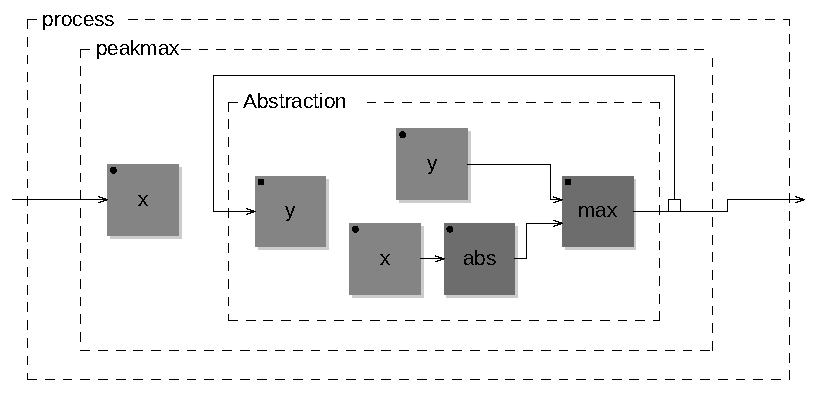
\includegraphics[width=12cm]{figures/PeakholderIIR.pdf} \\
    {Algoritmo e Schema del \textit{Peakholder} ad 1 campione di ritardo} \\ 
    \end{center}
    \begin{lstlisting}
        //---------------------------------------------------------- FAUST CODE
        import("stdfaust.lib");
        
        // LAR with Peak Max - IIR filter and max comparison
        peakmax = loop
        with{
            loop(x) = \(y).((y , abs(x)) : max)~_;
        };
        
        LARpeakmax = _ <: (_ * (1 - (_ : peakmax)));
        process = _ : LARpeakmax;
        //---------------------------------------------------------------------
    \end{lstlisting}
\begin{center}
    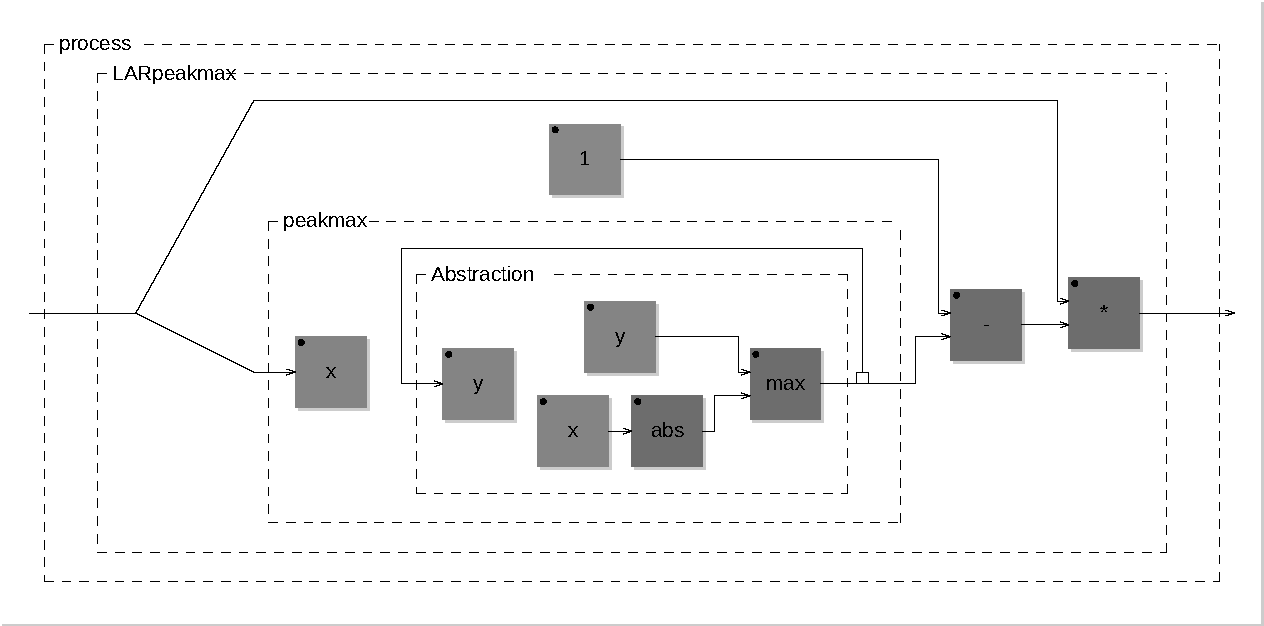
\includegraphics[width=12cm]{figures/LARpeakmax.pdf} \\
    {Algoritmo e Schema del LAR con \textit{Peakholder} ad 1 campione di ritardo} \\ 
\end{center}
\vspace{0.5cm}

Questo tipo di algoritmo presenta comunque alcuni problemi: non avendo
una funzione di smoothing del segnale, si verificano problemi di segnali di differenza a banda
molto larga che possono generare aliasing e contributi spuri che tendono a permanere nel
segnale complessivo.
Oltre a questo, variazioni del comportamento del Feedback sono dipendenti dalla grandezza
della finestra di osservazione, da eventuali cofficenti di feedback inseriti nella
retroazione del \textit{Peakholder} e da altri tipi di implementazioni di tecniche 
\textit{amplitude-following}. \\
Il meccanismo LAR è essenzialmente nel cuore della live performance del Feedback Study,
senza di questo non sarebbe possibile creare una condizione favorevole per procedere alle 
conseguenti trasformazioni del suono, ed ad una condizione favorevole affinché il 
sistema possa osservarsi tramite l'ambiente circostante. 
In tal senso vale la pena procedere osservando da vicino come viene richiesto in partitura 
di implementare questo meccanismo.

\begin{center}
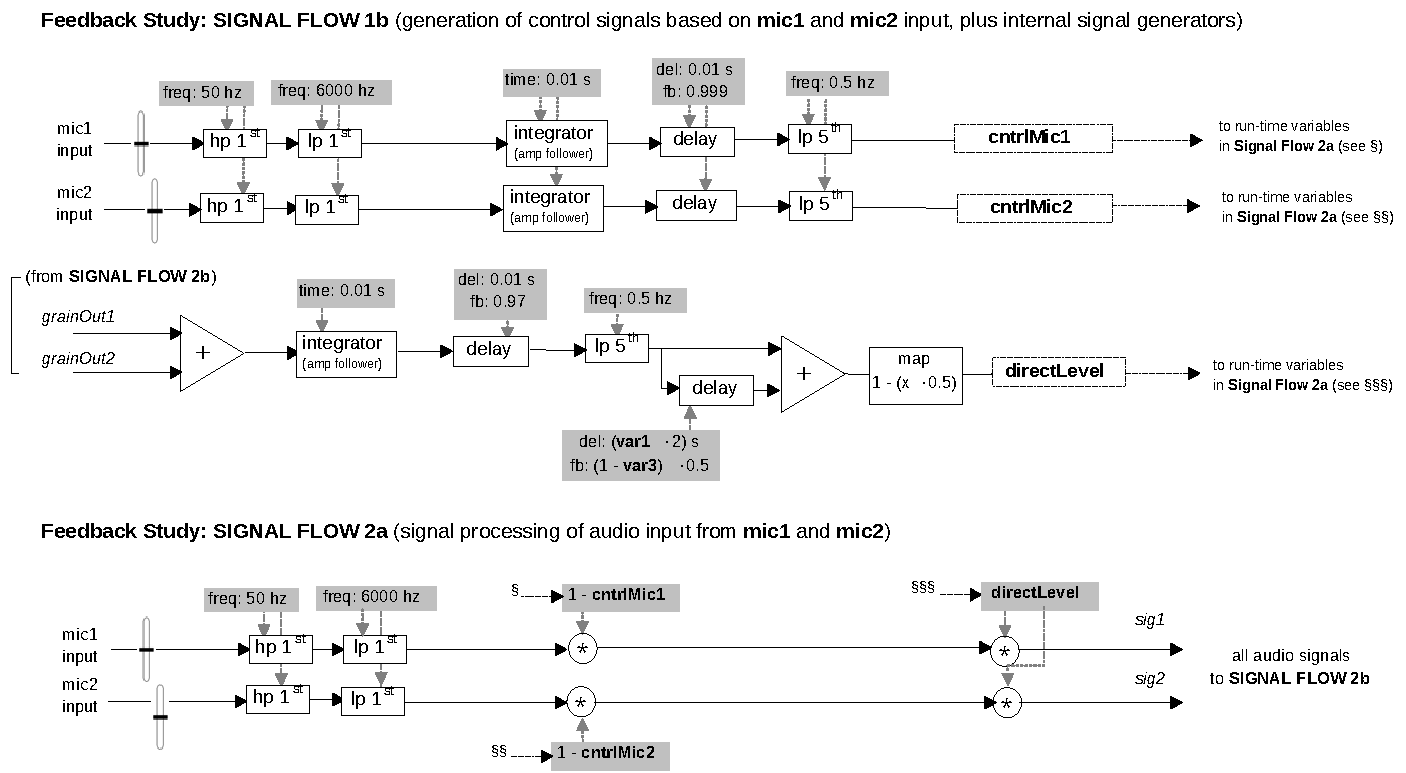
\includegraphics[width=14cm]{figures/LARfeedbackstudy2017.pdf} \\
{Estratto dalla partitura di \textit{Audible Ecosystemics n.2/ Feedback Study (2003)} \\
revisione del 2017 - Agostino Di Scipio} \\ 
\vspace{0.5cm}
\end{center}

Nel SIGNAL FLOW 1b,
due microfoni in ingresso (mic1 e mic2) vengono limitati in banda da un filtro Highpass ed 
un filtro Lowpass, rispettivamente fra 50 e 6000 Hz; dei due microfoni che escono 
dal cntrlMic1 e cntrlMic2 ne viene ricavato l'inviluppo d'ampiezza tramite
l'oggetto \textit{integrator}, poi la curva di questo inviluppo viene amplificata da 
un delay con Feedback, e ne viene estratta solamente la componente energetica 
presente fra i 0 e i 0.5Hz, limitandone il comportamento dell'oscillazione in quel range.
Più in basso, nel SIGNAL FLOW 2a, i stessi microfoni (mic1 e mic2) sempre
limitati in banda fra 50 e 6000 Hz, vengono attenuati in ampiezza dal segnale
proveniente dal cntrlMic1 e cntrlMic2, realizzando nella sostanza una 
versione più sofisticata del controbilanciamento del meccanismo LAR.
La parte restante: ovvero, la generazione del segnale directLevel e la 
conseguente attenuazione dei segnali audio in uscita (sig1 e sig2),
consiste in un secondo controbilanciamento ricavato da un processo di granulazione
attivo alla fine del sistema, finché il granulatore non produce segnale in output 
l'ampiezza dei segnali audio diretti in uscita dal sistema rimane inalterata. \\
L'inviluppo d'ampiezza ricavato tramite l'oggetto \textit{integrator}, in partitura 
viene richiesto come segue:

\begin{center}
    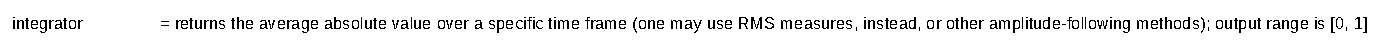
\includegraphics[width=14cm]{figures/integratorae2.pdf} \\
    {indicazioni specifiche riguardo l'oggetto \textit{integrator}} \\
    \vspace{0.5cm}
    \end{center}

dove sostanzialmente, viene calcolato il valore assoluto di una specifica finestra temporale. 
Viene indicato all'esecutore di poter utilizzare diversi metodi per poter calcolare il valore, come ad esempio l'RMS, 
tuttavia da analisi dirette sull'implementazione del compositore, i filtri utilizzati risultano essere di tipo IIR,
così da avere sostanzialmente una risposta più lenta rispetto ad altre tecniche come ad esempio quella del calcolo a media mobile.  
La risposta del filtro nell'implementazione originale è di tipo \textit{tau} e l'inviluppo è assoluto.